\chapter{数据库存储}

\section{存储介质}

\begin{figure}[H]
    \centering
    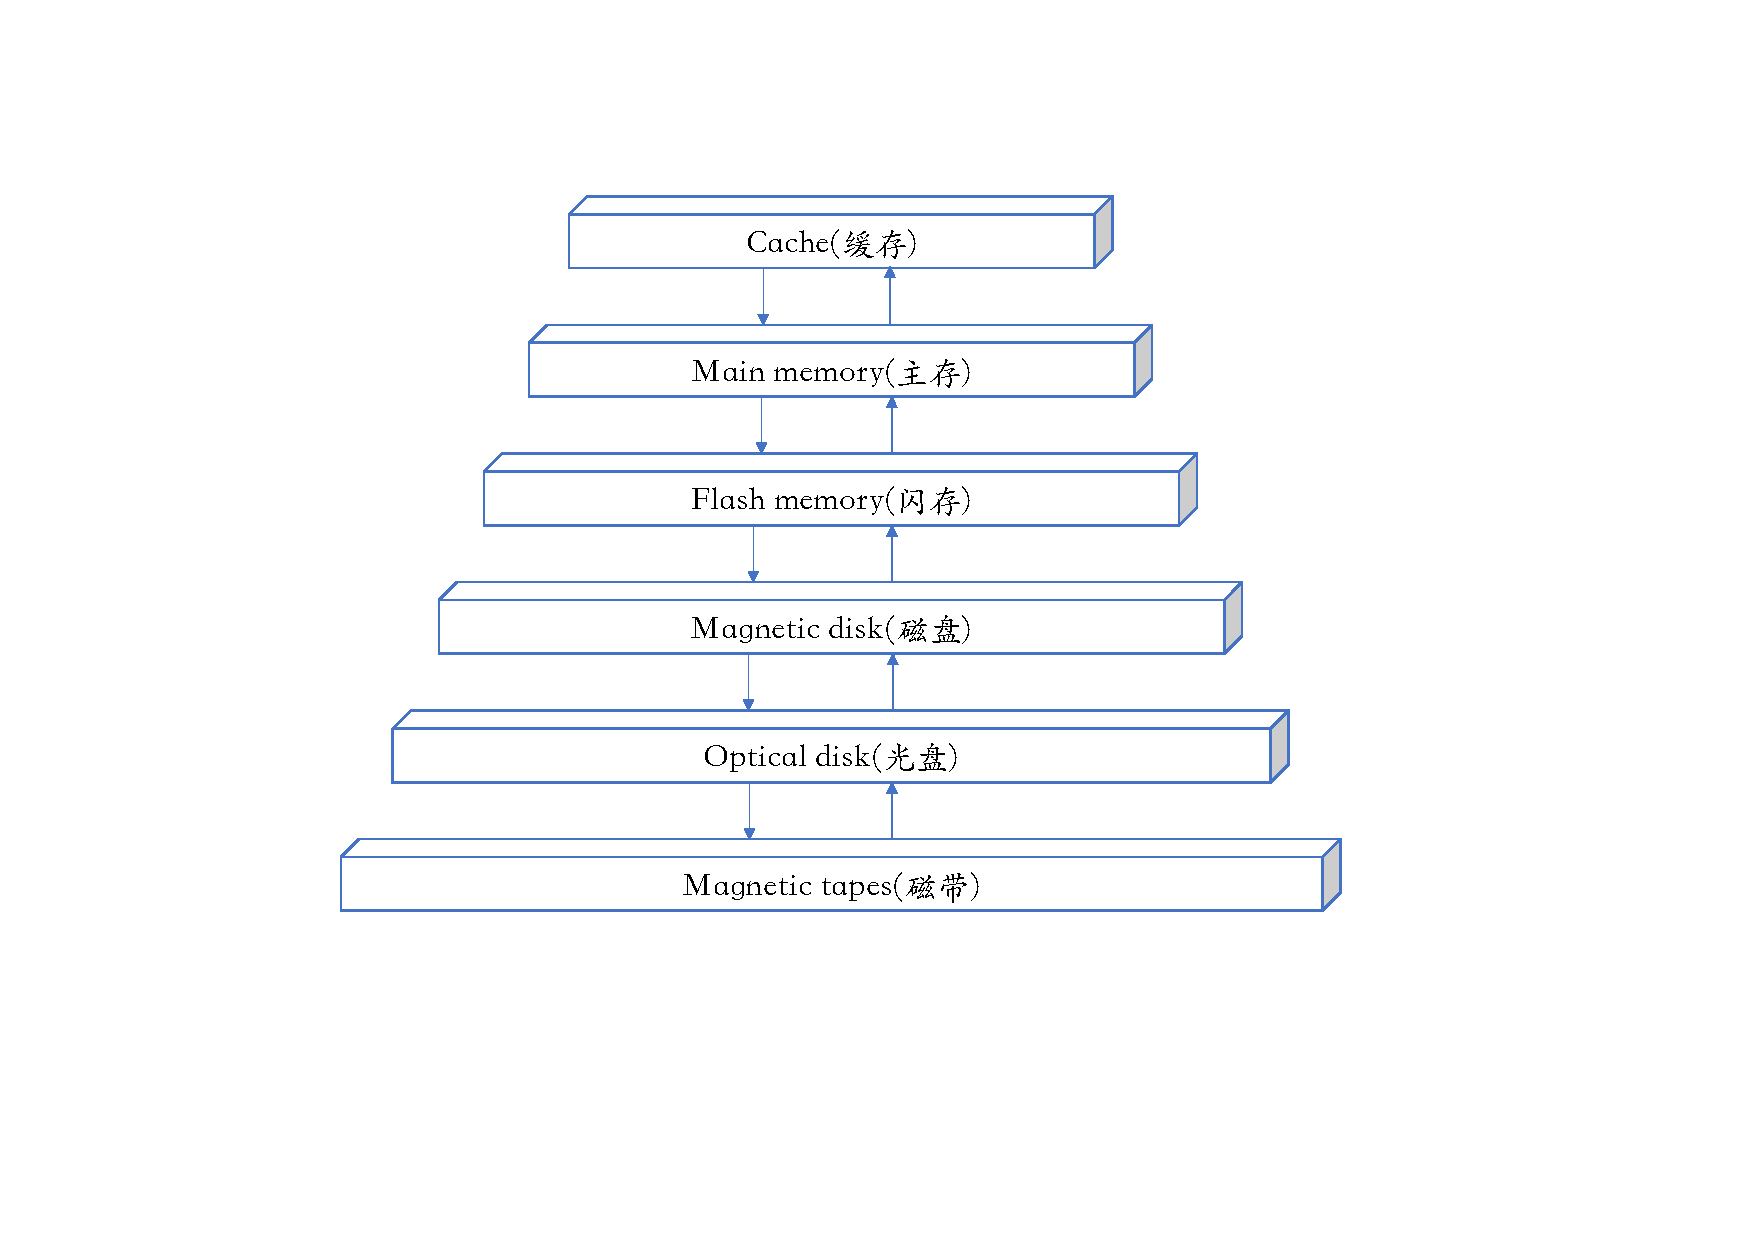
\includegraphics[width=.65\textwidth]{./figure/存储介质层次.pdf}
    \caption{物理存储介质的层次}
\end{figure}

局部性原理: CPU访问存储器时, 无论是存取指令还是存取数据, 所访问的存储单元都趋于聚集在一个较小的连续区域中.

